\section{System Architecture Overview}

This section provides an overview of the architecture of our indoor navigation system, designed to assist visually impaired users with real-time, context-aware guidance within indoor environments. The system leverages mobile technology, backend services, and sensory input devices to deliver seamless and accessible navigation. Below, we briefly introduce the key components and their roles, supported by a use case diagram and system architecture illustration.

\subsection{High-Level View of Components}

The system comprises four main components, each explained briefly below. Detailed descriptions of each component are provided in subsequent sections.

\begin{itemize}
	\item \textbf{Mobile Application}: The mobile application acts as the central interface for users and the processing unit for the system. It facilitates QR code scanning, provides navigation instructions via TalkBack, processes obstacle detection data, and communicates with the backend server to retrieve location-specific data. The app also enables users to connect the IO components they want. This is done by choosing th desired camera, microphone, and sound output devices from the settings. The default devices will be the ones on the phone.
	
	\item \textbf{Localization System}: The localization system determines the user’s global position and orientation within the environment. It uses QR code scanning and positional data retrieval from the backend to calculate the user’s current position relative to the environment.
	
	\item \textbf{Customizable Guidance System}: The guidance system provides real-time navigation assistance by retrieving and delivering location-based instructions. It allows users to select destinations and offers step-by-step guidance through TalkBack, dynamically updating as the user progresses along the path.
	
	\item \textbf{Obstacle Detection System}: The obstacle detection system ensures safety by alerting users to nearby obstacles. Using four ultrasonic sensors and vibration motors, it delivers tactile feedback proportional to the proximity of detected obstacles, enhancing the user's awareness of their surroundings.


	\item \textbf{Building Management Dashboard}: The Building Management Dashboard provides secure authentication for administrators to access and manage their building layouts, including all QR codes within the building. It allows them to edit instructions, generate printable QR codes, and perform bulk updates to instructions across a floor, section, or the entire building efficiently.
	
\end{itemize}

\subsection{Use Case Diagram}

The following use case diagram (see Figure~\ref{fig:use_case_diagram}) illustrates the interactions between the users and the system components, including QR code data retrieval, QR code management, customization guidance, localization, and obstacle detection:

\begin{figure}[h]
	\centering
	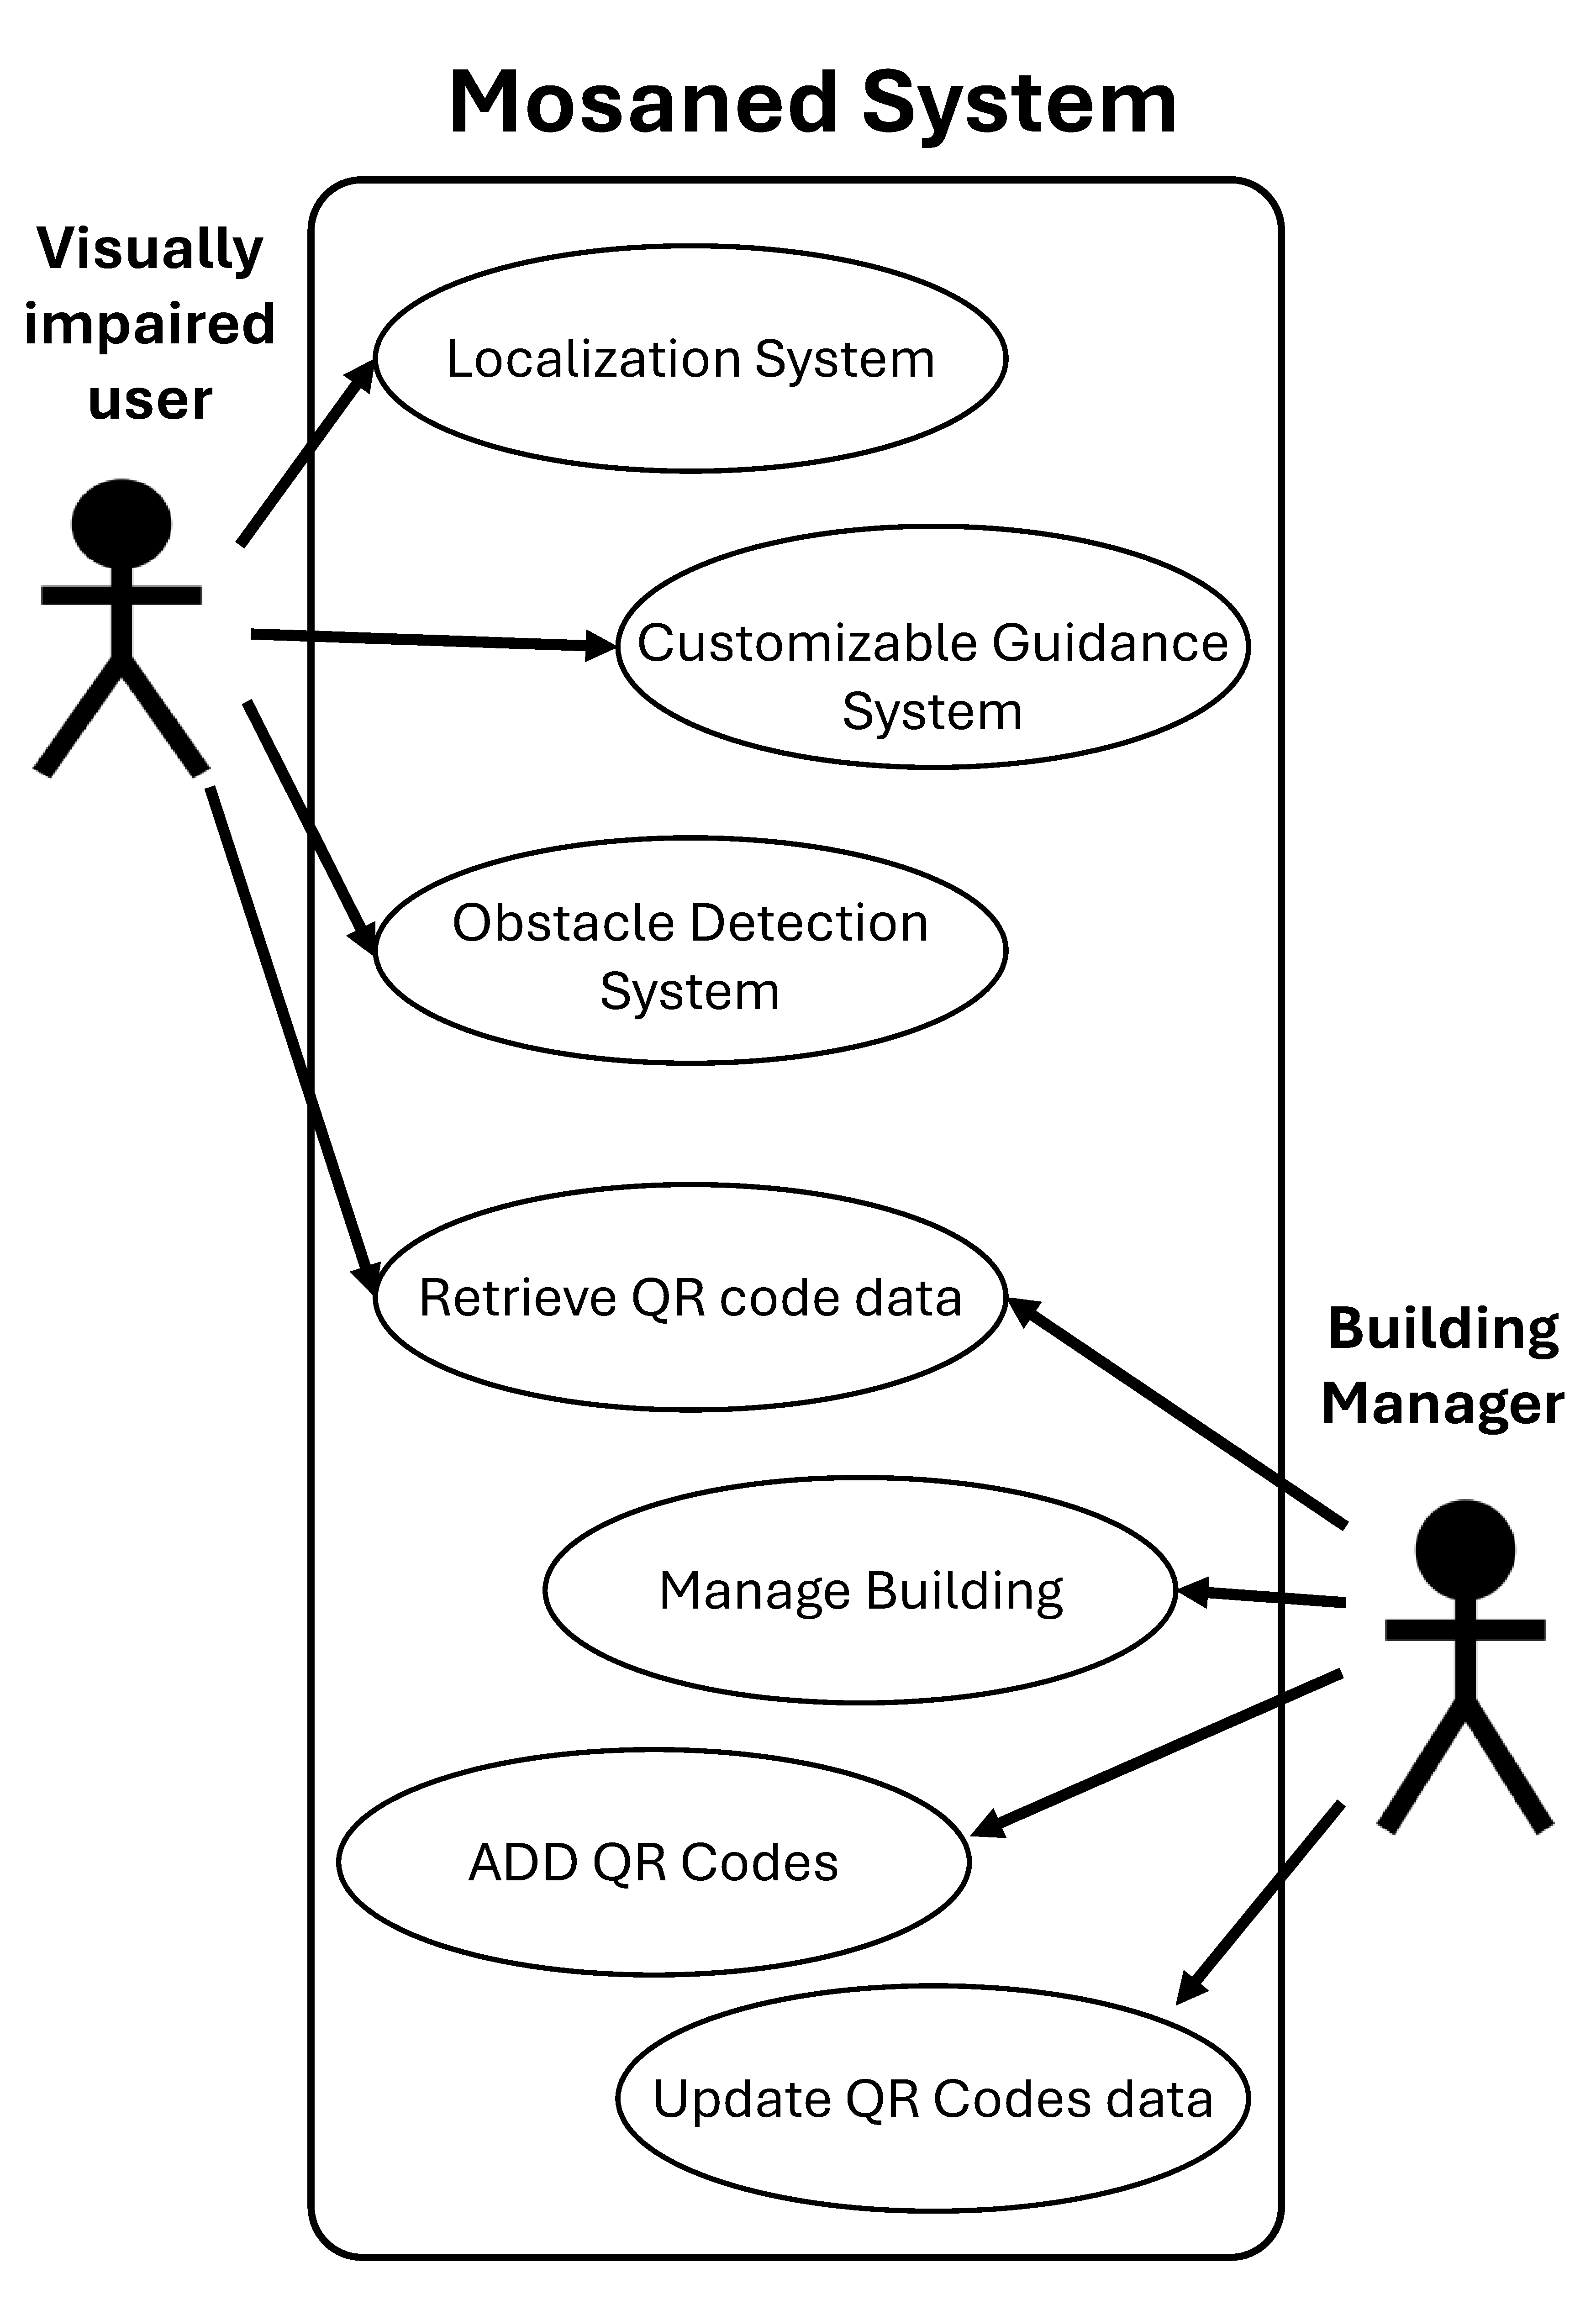
\includegraphics[width=0.6\linewidth]{assets/ch2/use_case}
	\caption{Use Case Diagram of Mosaned System}
	\label{fig:use_case_diagram}
\end{figure}

\subsection{System Architecture Diagram}

The system architecture diagram (see Figure~\ref{fig:system_architecture}) provides a high-level view of how the components are connected and interact, where the arrows show the flow of data. 

\begin{figure}[h]
	\centering
	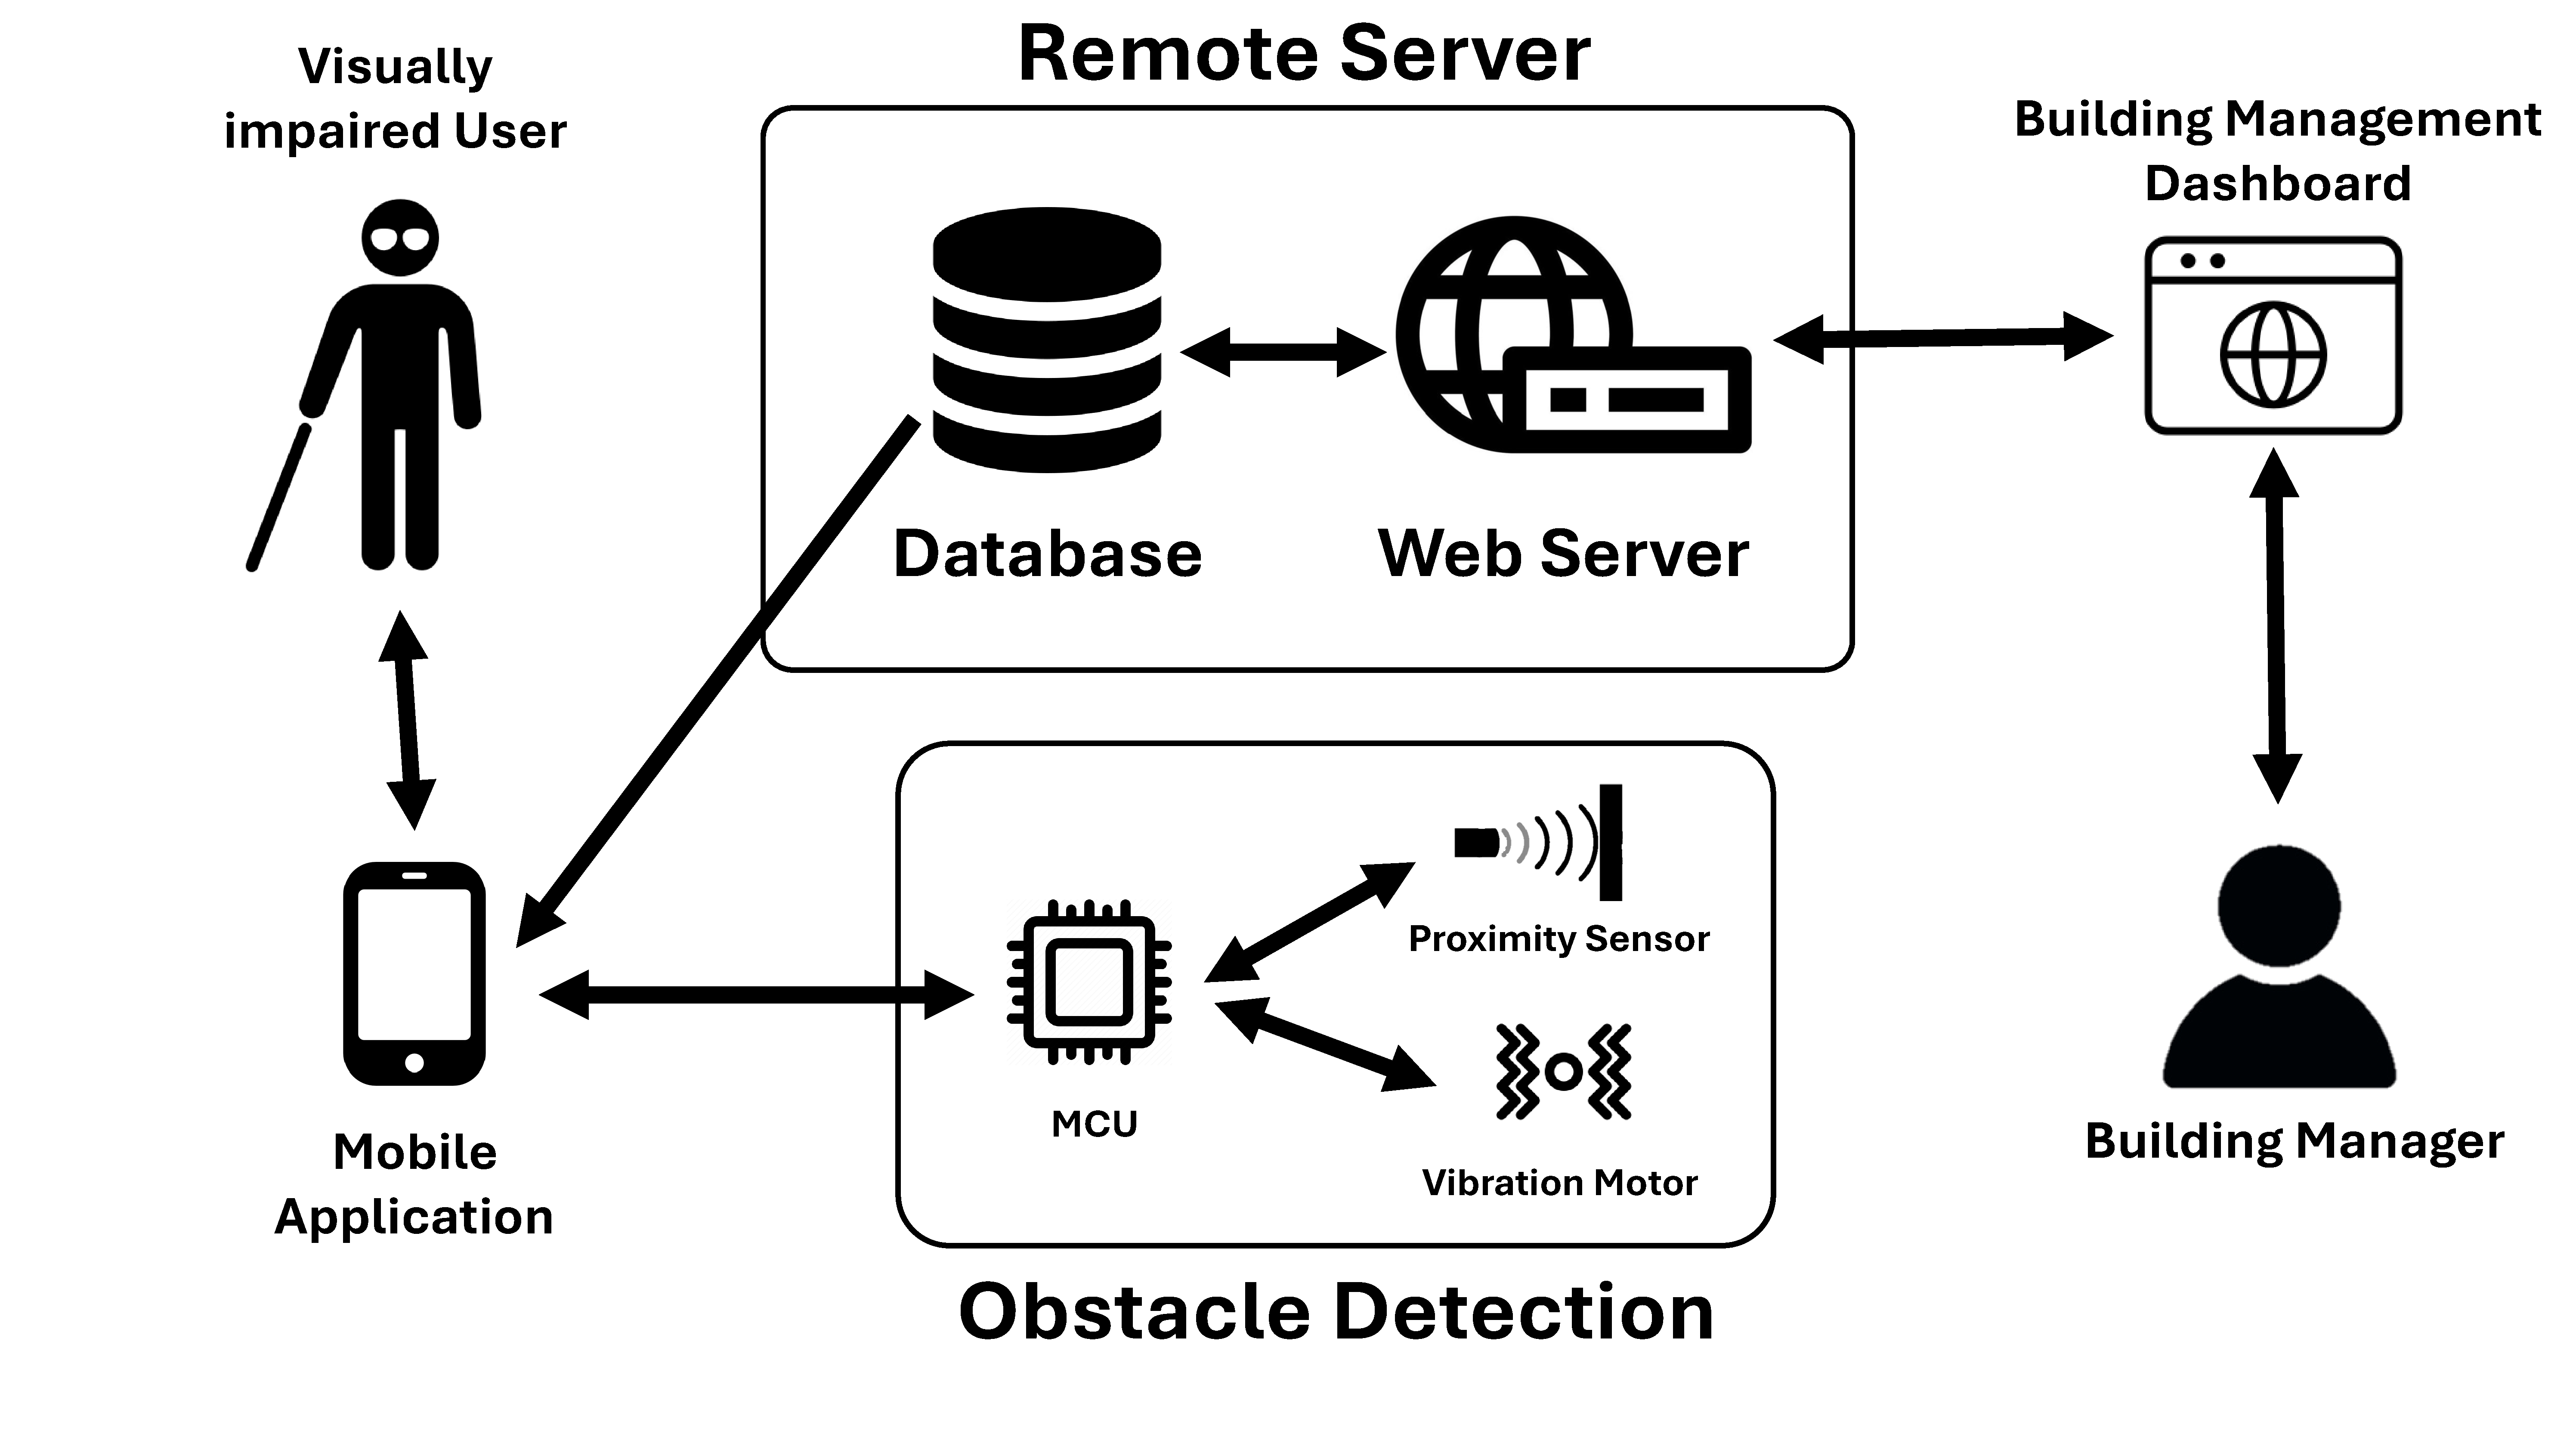
\includegraphics[width=1\linewidth]{assets/ch2/sys_arch}
	\caption{System Architecture Diagram of Mosaned System}
	\label{fig:system_architecture}
\end{figure}

This high-level overview introduces the core components and their functions within the system. Subsequent sections provide detailed explanations of each component, their implementation, and integration.
